% Задание

% 1. Описать принципиальную схему работы ПО с акцентом на методы защиты информации.
% 2. Перечислить используемые (возможные к использованию) алгоритмы шифрования и контроля целостности.
% Указать механизм применения пароля/ключа в процессе шифрования пользовательских данных и
% (при необходимости) дополнительные параметры, влияющие на процесс.
% 3. Описать структуру файла-контейнера.
% 4. Проверить работу ПО на тестовых входных данных, продемонстрировать структуру результирующих файлов-контейнеров.
% 5. Описать (при наличии) известные уязвимости (CWE, CVE) ПО на базе cvedetails.com и/или аналогичных банков уязвимостей.
% 6. Результаты работы представить в формате LaTeX.

\documentclass[12pt,a4paper]{article}
\usepackage[T1,T2A]{fontenc}
\usepackage[english,russian]{babel}
\usepackage[margin=2.5cm]{geometry}
\usepackage[utf8]{inputenc}

\usepackage{amsmath}
\usepackage{array}
\usepackage{booktabs}
\usepackage{caption}
\usepackage{float}
\usepackage{graphicx}
\usepackage{hyperref}
\usepackage{listings}
\usepackage{multirow}
\usepackage{parskip}
\usepackage{tabularx}
\usepackage{xcolor}
\usepackage{subcaption}
\usepackage{wrapfig}

\addto\captionsrussian{
  \renewcommand{\figurename}{Рисунок}
}

\lstset{
    basicstyle=\small\ttfamily,
    breaklines=true,                 % Wraps long lines
    breakatwhitespace=true,          % Only wraps at spaces to keep it readable
    showstringspaces=false,          % Removes "cup" symbols in strings
    showspaces=false,                % Removes "cup" symbols in general
    postbreak=\mbox{\textcolor{gray}{$\hookrightarrow$}\space}, % Visual wrap indicator
    columns=fullflexible,            % Improves character spacing
    frame=single,                    % Optional: adds a box around the code
    % Support for special characters like ©
    literate={©}{{\textcopyright}}1
}

\title{\textbf{Утилита шифрования файлов Cloaker}\\
       \large Отчёт по анализу безопасности}
\author{Klixel}
\date{\today}

\begin{document}

\maketitle
\newpage
\tableofcontents
\newpage

\section{Принципиальная схема работы ПО}

Cloaker --- это утилита для симметричного шифрования файлов с использованием пароля, заданного пользователем.

Репозиторий проекта состоит из четырёх основных компонент:
\begin{itemize}
    \item \textbf{core} --- библиотека, в которой реализованы функции шифрования и дешифрования данных, а также функции для взаимодействия с файловой системой и управления параметрами утилиты.
    \item \textbf{gui} --- графический интерфейс, позволяющий пользователю легко и интуитивно взаимодействовать с функционалом утилиты с помощью технологии drag-and-drop.
    \item \textbf{cli} --- интерфейс командной строки, предоставляющий возможность использовать утилиту в терминале для более продвинутой настройки параметров и автоматизации процессов шифрования.
    \item \textbf{adapter} --- статическая библиотека, которая обеспечивает взаимодействие между \textbf{core}, написанном на языке программирования Rust, и графическим интерфейсом, написанным на языке C++ с использованием фреймворка Qt.
\end{itemize}

\subsection{Обзор \texttt{core}}

Библиотека \textbf{core} предоставляет публичные структуры для настройки параметров шифрования, функции для обработки файлов, функцию для шифрования данных, а также современную и устаревшую реализацию функции дешифрования данных. Устаревшая реализация сохранена для обеспечения обратной совместимости с старой структурой файла-контейнера, которая использовалась в предыдущих версиях утилиты.

\subsection*{Процесс шифрования предоставленных данных}

Функция шифрования принимает на вход ссылки на потоки для чтения и записи, заданный пользователем пароль, указатель на Ui для отображения прогресса в пользовательских интерфейсах, а также размер входящих данных.

Процесс шифрования включает следующие этапы:
\begin{enumerate}
    \item ПО записывает в выходной поток заголовок \texttt{0xC10A6BED}, который служит для идентификации современного формата файла-контейнера.
    \item ПО генерирует псевдослучайную криптографически безопасную соль длиной 128 бит (16 байт) с помощью функции \texttt{argon2id13::gen\_salt()} и записывает её в выходной поток.
    \item На основе введённого пользователем пароля и сгенерированной соли алгоритм \texttt{Argon2id} с параметрами \texttt{opslimit = 2} и \texttt{memlimit = 67108864} (64 Мб) создаёт 256-битный ключ шифрования.
    \item Ключ шифрования используется для инициализации алгоритма аутентифицированного шифрования \texttt{XChaCha20-Poly1305}, который обеспечивает конфиденциальность и аутентичность данных. На основе ключа, алгоритм генерирует 192-битный (24 байтный) вектор инициализации, который также записывается в выходной поток.
    \item Входной файл читается блоками по 512 КБ. Каждый блок шифруется с помощью алгоритма \texttt{XChaCha20-Poly1305}, после чего результат записывается в выходной поток вместе с 16-байтной имитовставкой, которая служит для проверки целостности данных при дешифровании, и байтом, указывающим на наличие следующего блока данных. \\
    Процесс повторяется до тех пор, пока весь входной файл не будет обработан.
\end{enumerate}

\subsection*{Процесс дешифрования предоставленных данных}

Обе функции дешифрования принимают на вход ссылки на потоки для чтения и записи, заданный пользователем пароль, указатель на Ui для отображения прогресса в пользовательских интерфейсах и размер входящих данных. Устаревшая реализация функции также принимает на вход массив с первыми 4 байтами входного потока для их дальнейшего сравнения с заголовком файла-контейнера.

Процесс дешифрования можно описать следующим образом:
\begin{enumerate}
    \item Функция дешифрования проверяет, что размер входящих данных не меньше минимального размера, который может содержать валидный файл-контейнер. Если размер данных меньше, функция возвращает ошибку.
    \item Функции извлекают из входного потока заголовок (если он есть), соль и вектор инициализации. Соль и переданный пользователем пароль используются для генерации ключа шифрования с помощью алгоритма \texttt{Argon2id} (в новом формате) или \texttt{scrypt} (в старом формате).
    \item Ключ шифрования и вектор инициализации используются для инициализации алгоритма \texttt{XChaCha20-Poly1305}.
    \item Входной файл читается блоками по (512 * 1024 + 17) байт. Каждый блок дешифруется с помощью алгоритма \texttt{XChaCha20-Poly1305}, после чего его целостность проверяется с помощью сравнения с имитовставкой. Если проверка не проходит, функция возвращает ошибку. Если проверка проходит, результат записывается в выходной поток. Процесс повторяется до тех пор, пока весь входной файл не будет обработан.
\end{enumerate}

\newpage

\subsection{Обзор \texttt{gui}}

\begin{wrapfigure}{r}{0.35\textwidth} % 'r' for right side, width of the wrapping box
    \centering
    \vspace{-10pt} % Adjusts top spacing so it aligns perfectly with the first line of text
    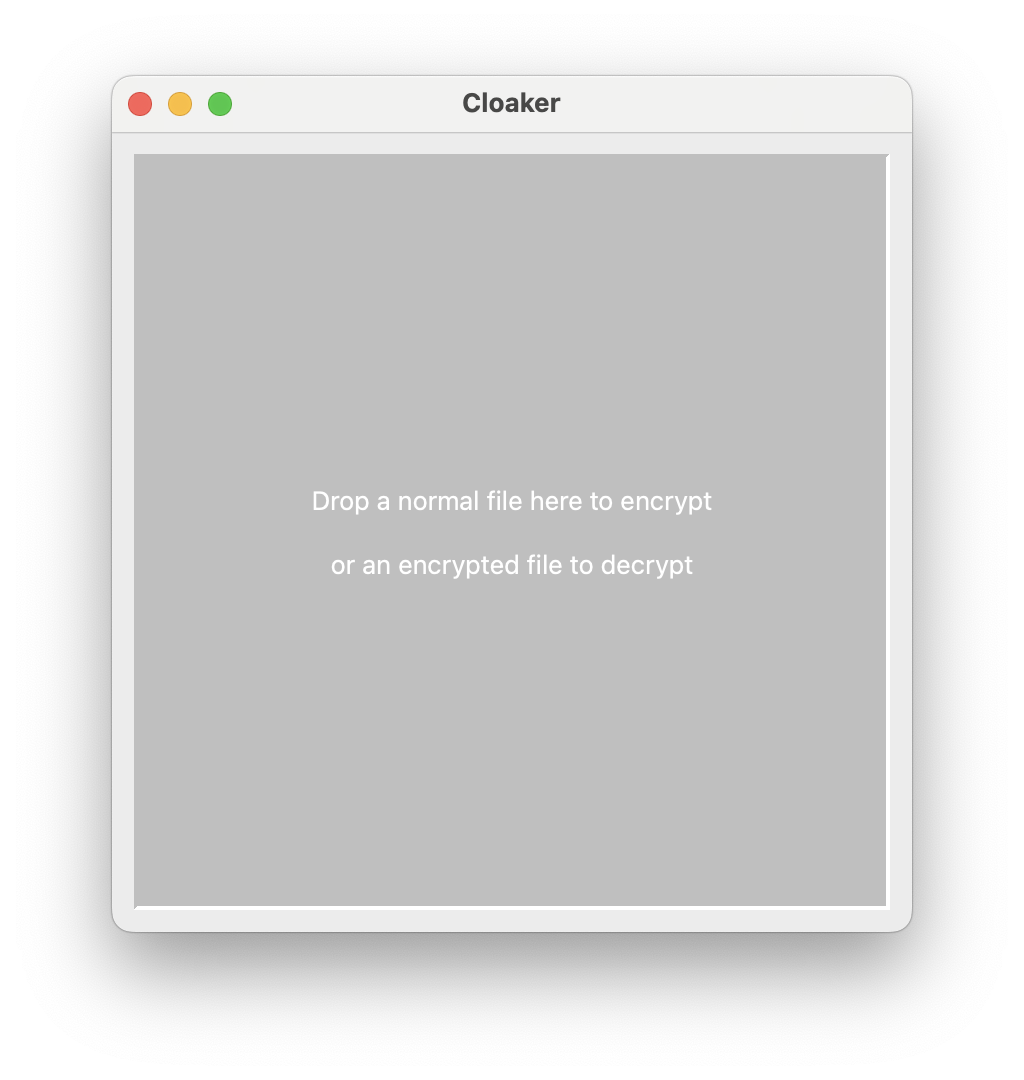
\includegraphics[width=0.3\textwidth]{GUI_interface.png}
    \caption{Окно приложения}
    \label{interface}
    \vspace{-10pt} % Reduces empty space below the figure
\end{wrapfigure}

Графический интерфейс \textbf{gui} написан на языке программирования C++ с использованием фреймворка Qt. Он предоставляет собой окно, в которое пользователь может перетаскивать файлы для их шифрования или дешифрования (\autoref{interface}).

Когда пользователь перетаскивает файл в окно, интерфейс определяет, является ли файл зашифрованным или нет с помощью сравнения первых 4 байт файла с современным заголовком \texttt{0xC10A6BED} и устаревшим заголовком \texttt{0xC10A4BED}, а также проверки расширения файла на совпадение с расширением \texttt{.cloaker}.

\subsection*{Шифрование файла}

Если файл не является зашифрованным, интерфейс запрашивает у пользователя пароль длиной 12 и более символов для шифрования файла (\autoref{fig:enter_password}).

После ввода пароля, интерфейс запрашивает у пользователя подтверждение пароля для предотвращения ошибок при вводе (\autoref{fig:confirm_password}). Если подтверждение не совпадает с первоначальным вводом, интерфейс отображает сообщение об ошибке и запрашивает пароль снова (\autoref{fig:dont_match}).

Если подтверждение совпадает, интерфейс предлагает пользователю выбрать название и расположение для сохранения зашифрованного файла (\autoref{fig:save_file}). После этого интерфейс вызывает функцию шифрования из библиотеки \textbf{core}. При этом интерфейс отображает прогресс шифрования с помощью прогресс-бара, который обновляется после обработки каждого блока данных. После завершения процесса шифрования, интерфейс отображает сообщение об успешном завершении операции (\autoref{fig:success}).

% === FIRST PART OF THE FIGURE (Fits on current page) ===
\begin{figure}[H]
    \centering
    \begin{subfigure}{0.3\textwidth}
        \centering
        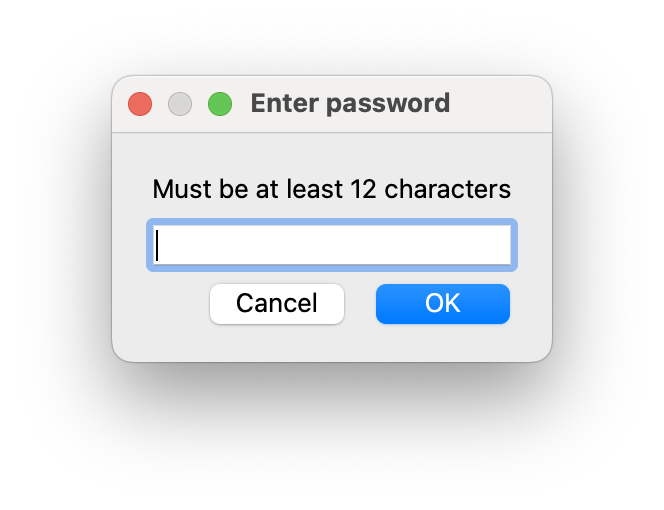
\includegraphics[width=\linewidth]{Enter_password.png}
        \caption{Ввод пароля}
        \label{fig:enter_password}
    \end{subfigure}\hfill
    \begin{subfigure}{0.3\textwidth}
        \centering
        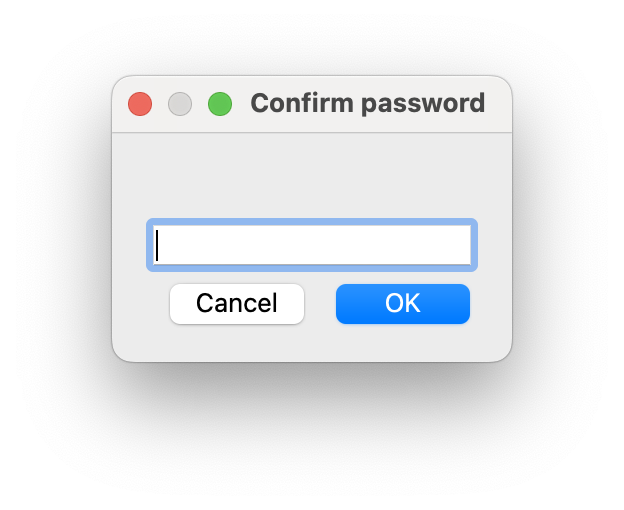
\includegraphics[width=\linewidth]{Confirm_password.png}
        \caption{Подтверждение}
        \label{fig:confirm_password}
    \end{subfigure}\hfill
    \begin{subfigure}{0.3\textwidth}
        \centering
        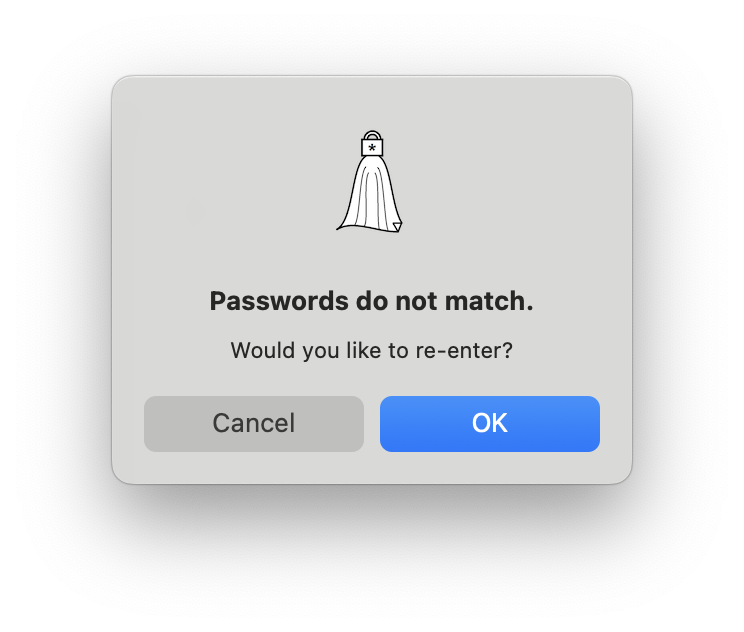
\includegraphics[width=\linewidth]{Passwords_dont_match.png}
        \caption{Ошибка ввода}
        \label{fig:dont_match}
    \end{subfigure}
    \caption{Формы взаимодействия с пользователем при шифровании (часть 1)}
    \label{fig:gui_forms_part1}
\end{figure}

% === SECOND PART OF THE FIGURE (Flows to the next page) ===
\begin{figure}[H]
    \ContinuedFloat
    \centering
    \begin{subfigure}{0.3\textwidth}
        \centering
        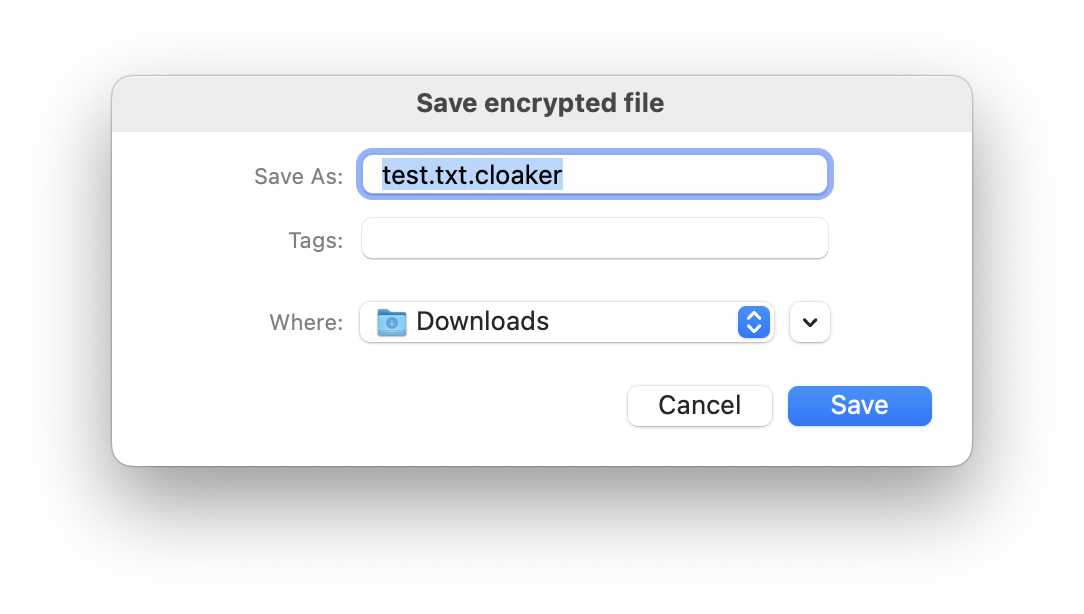
\includegraphics[width=\linewidth]{Save_file.png}
        \caption{Выбор названия}
        \label{fig:save_file}
    \end{subfigure}\hspace{0.05\textwidth}
    \begin{subfigure}{0.3\textwidth}
        \centering
        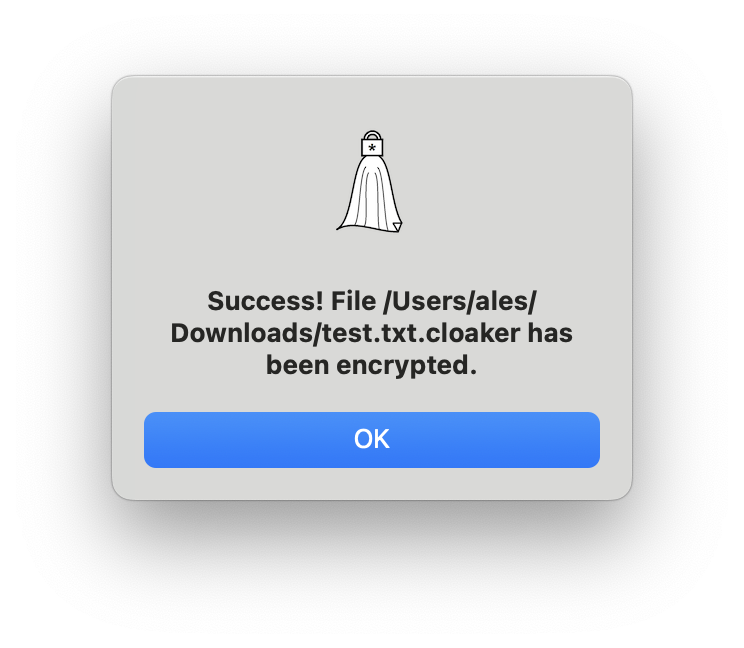
\includegraphics[width=\linewidth]{Success.png}
        \caption{Успешное шифрование}
        \label{fig:success}
    \end{subfigure}
    \caption{Формы взаимодействия с пользователем при шифровании (часть 2)}
    \label{fig:gui_forms} % This label can be used to reference the whole group
\end{figure}

\subsection*{Дешифрование файла}

Если файл является зашифрованным, интерфейс запрашивает у пользователя пароль для дешифрования файла (\autoref{fig:decrypt_password}) и предлагает выбрать название и расположение для сохранения дешифрованного файла (\autoref{fig:save_decrypted}).
После этого интерфейс вызывает функцию дешифрования из библиотеки \textbf{core}. При этом интерфейс отображает прогресс дешифрования с помощью прогресс-бара, который обновляется после обработки каждого блока данных. Если в процессе дешифрования возникает ошибка (например, из-за неправильного пароля или повреждённого файла), интерфейс отображает сообщение об ошибке (\autoref{fig:decrypt_fail}) и файл для записи удаляется. Если процесс завершается успешно, интерфейс отображает сообщение об успешном завершении операции (\autoref{fig:decrypt_success}).

\begin{figure}[H]
    \centering
    \begin{subfigure}{0.3\textwidth}
        \centering
        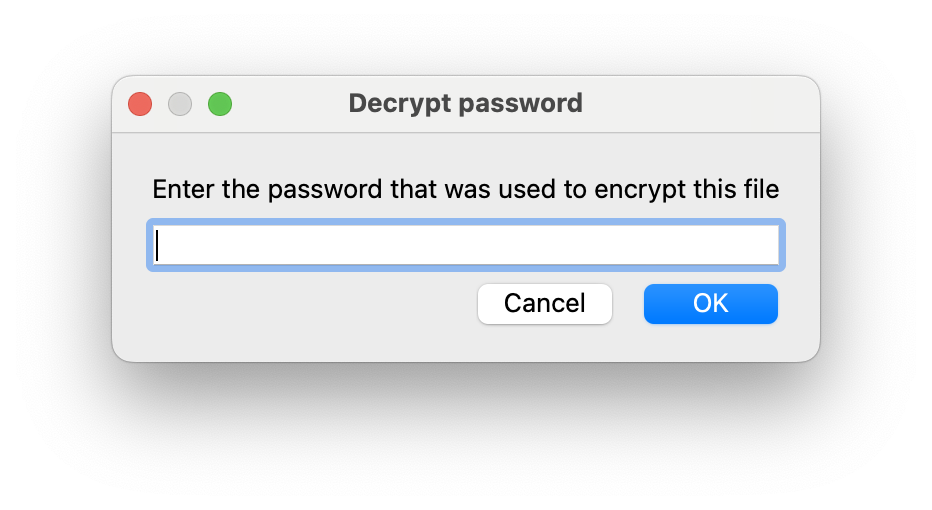
\includegraphics[width=\linewidth]{Decrypt_password.png}
        \caption{Ввод пароля}
        \label{fig:decrypt_password}
    \end{subfigure}\hspace{0.1\textwidth}
    \begin{subfigure}{0.3\textwidth}
        \centering
        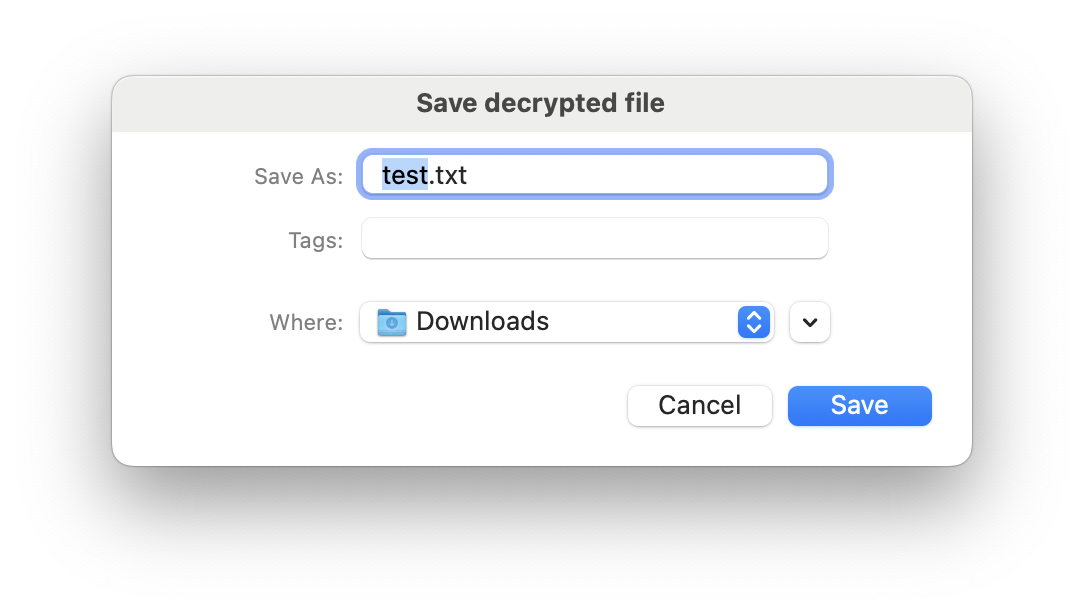
\includegraphics[width=\linewidth]{Save_decrypted.png}
        \caption{Выбор названия}
        \label{fig:save_decrypted}
    \end{subfigure}

    \vspace{1.5em} % Adds vertical breathing room between rows

    \begin{subfigure}{0.3\textwidth}
        \centering
        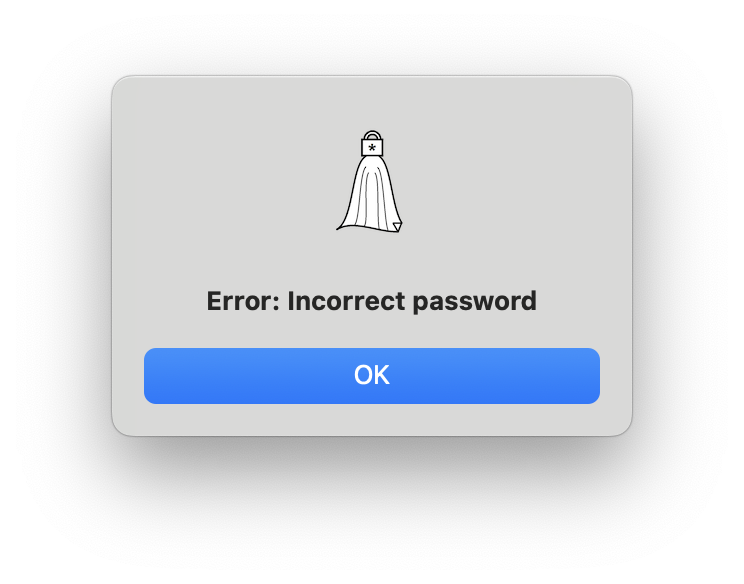
\includegraphics[width=\linewidth]{Incorrect_password.png}
        \caption{Ошибка дешифровки}
        \label{fig:decrypt_fail}
    \end{subfigure}\hspace{0.1\textwidth}
    \begin{subfigure}{0.3\textwidth}
        \centering
        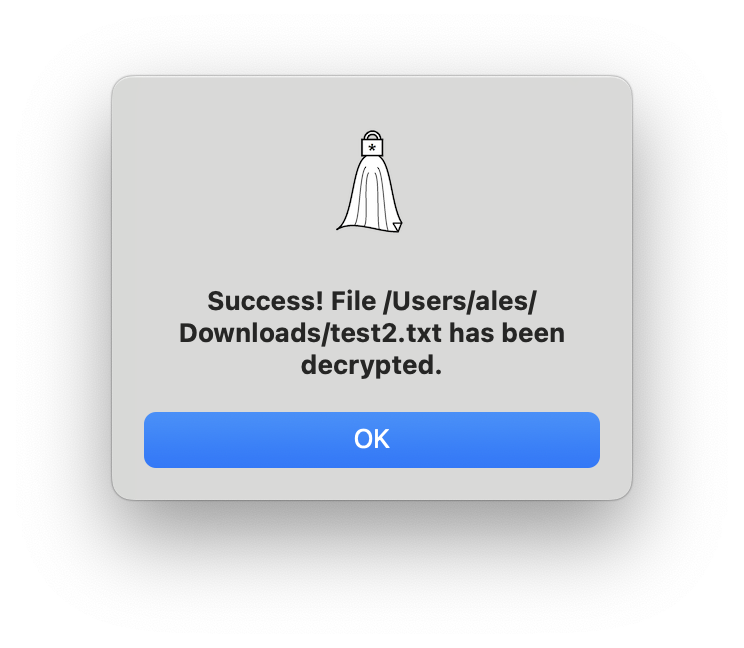
\includegraphics[width=\linewidth]{Decrypt_success.png}
        \caption{Успешная дешифровка}
        \label{fig:decrypt_success}
    \end{subfigure}
    \caption{Формы взаимодействия с пользователем при дешифровании}
    \label{fig:gui_forms_decrypt}
\end{figure}

\newpage

\subsection{Обзор \texttt{cli}}

Интерфейс командной строки \textbf{cli} предоставляет пользователю возможность использовать утилиту в терминале для более продвинутой настройки параметров и автоматизации процессов шифрования и дешифрования.

Справочная информация об использовании интерфейса:
\begin{lstlisting}[language=bash]
% ./cloaker_cli --help
Cloaker v4.0
Theron Spiegl
Cloaker is a simple file encryption utility. Passwords must be at least 12 characters, though longer is better. Written
in Rust using sodiumoxide/libsodium's secretstream encryption. Copyright © 2021 Theron Spiegl. All rights reserved.
https://cloaker.spiegl.dev/

USAGE:
    cloaker_cli [FLAGS] [OPTIONS] <--encrypt <FILE_TO_ENCRYPT>|--decrypt <FILE_TO_DECRYPT>|--encrypt-stdin|--decrypt-stdin>

FLAGS:
    -D, --decrypt-stdin
                    Decrypt from stdin instead of a file. If an output filename is not specified with -o, the default will be `./decrypted_stdin`.
    -E, --encrypt-stdin
                    Encrypt from stdin instead of a file. If an output filename is not specified with -o, the default will be `./encrypted.cloaker`.
    -h, --help
                    Prints help information
    -O, --stdout
                    Encrypt or decrypt to stdout instead of to a file.
    -V, --version
                    Prints version information

OPTIONS:
    -d, --decrypt <FILE_TO_DECRYPT>
                    Specifies the file to decrypt.
    -e, --encrypt <FILE_TO_ENCRYPT>
                    Specifies the file to encrypt.
    -o, --output <PATH_TO_OUTPUT_FILE>
                    Specifies a path or name for the output file. If the path to an existing directory is given, the input filename will be kept with the .cloaker extension added if encrypting or removed (if decrypting). Otherwise the file will be placed and named according to this parameter.
\end{lstlisting}
\newpage
\begin{lstlisting}[language=bash]
    -p, --password <PASSWORD>
                    Optional, and not recommended due to the password appearing in shell history.
                    Password for the file. This or the --password-file (-f) flag is required if using stdin and/or stdout.
    -f, --password-file <PASSWORD_FILE>
                    The password to encrypt/decrypt with will be read from a text file at the path provided. File should be valid UTF-8 and contain only the password with no newline. This or the --password (-p) flag is required if using stdin and/or stdout.
\end{lstlisting}

Можно заметить, что в отличие от графического интерфейса, интерфейс командной строки предоставляет пользователю возможность указать пароль любой длины (в том числе и пустой) для шифрования и дешифрования данных и корректно обрабатывает такие случаи, не проверяя длину использованного пароля.

\begin{lstlisting}[language=bash]
% ./cloaker_cli -e test.txt -p "" -o test_txt_empty_password.cloaker
Encrypting: 100%
Success! test_txt_empty_password.cloaker has been encrypted.
% ./cloaker_cli -d test_txt_empty_password.cloaker -o test_no_password.txt
Password:
Decrypting: 100%
Success! test_no_password.txt has been decrypted.
% ./cloaker_cli -d test_txt_empty_password.cloaker -o test_empty_password_incorrect_password.txt --password "test"
Error: Incorrect password
\end{lstlisting}

Также, с помощью интерфейса командной строки удобно показать различия в зашифрованных файлах из-за разной псевдослучайной соли даже при использовании одинакового пароля:

\begin{lstlisting}[language=bash]
% ./cloaker_cli -e test.txt -p "test_password" -o test1.cloaker
Encrypting: 100%
Success! test1.cloaker has been encrypted.
% ./cloaker_cli -e test.txt -p "test_password" -o test2.cloaker
Encrypting: 100%
Success! test2.cloaker has been encrypted.

% xxd -p -l 30 test1.cloaker | tr -d '\n' | sed 's/$/.../'; echo
c10a6bed942988c57a845e9cb4bc216e2e09cccd721185d7c2a35cf064f4...
% xxd -p -l 30 test2.cloaker | tr -d '\n' | sed 's/$/.../'; echo
c10a6bedda0aca33b1fb1dd1ea763188dca7bb7dc4a10b08333175b9ac81...
% openssl dgst -sha256 test1.cloaker
SHA2-256(test1.cloaker)= 1b0e886bdff38f2ebef38e018bdef98a93366fb0b7928fe854a6a1a123dd82c8
% openssl dgst -sha256 test2.cloaker
SHA2-256(test2.cloaker)= 42b3fd61708c9add111237cf4544c8c3fd1889f8564c6786941c29419ccf315c
\end{lstlisting}

Как видно по шестнадцатиричному представлению первых 30 байт обоих файлов, за исключением заголовка, файлы полностью различаются. Что также подтверждается хешем обоих файлов.

Однако, оба файла корректно дешифруются в файлы с одинаковым содержанием, совпадающим с изначальным файлом.

\begin{lstlisting}[language=bash]
% ./cloaker_cli -d test1.cloaker -p "test_password" -o test1_decrypted.txt
Decrypting: 100%
Success! test1_decrypted.txt has been decrypted.
% ./cloaker_cli -d test2.cloaker -p "test_password" -o test2_decrypted.txt
Decrypting: 100%
Success! test2_decrypted.txt has been decrypted.

% openssl dgst -sha256 test.txt
SHA2-256(test.txt)= d9014c4624844aa5bac314773d6b689ad467fa4e1d1a50a1b8a99d5a95f72ff5
% openssl dgst -sha256 test1_decrypted.txt
SHA2-256(test1_decrypted.txt)= d9014c4624844aa5bac314773d6b689ad467fa4e1d1a50a1b8a99d5a95f72ff5
% openssl dgst -sha256 test2_decrypted.txt
SHA2-256(test2_decrypted.txt)= d9014c4624844aa5bac314773d6b689ad467fa4e1d1a50a1b8a99d5a95f72ff5
\end{lstlisting}

Также я проверил изменение в работе утилиты при преобразовании заголовка из современного формата \texttt{0xC10A6BED} в устаревший формат \texttt{0xC10A4BED}, при изменении значений в соли, в теге блока с нуля на единицу и наоборот, в самом блоке данных.

Во всех случаях, утилита вернула ошибку "Error: Incorrect password", что свидетельствует о том, что утилита корректно обрабатывает случаи с некорректными данными и не позволяет дешифровать данные при изменении даже одного бита.

\begin{lstlisting}[language=bash]
% ./cloaker_cli -d file_with_modified_hex_values.cloaker -p "test_password" -o decrypted_file.txt

Error: Incorrect password
\end{lstlisting}

\subsection{Обзор \texttt{adapter}}

Статическая библиотека \textbf{adapter} написана на языке программирования Rust и обеспечивает взаимодействие между \textbf{core} и графическим интерфейсом \textbf{gui}. Она предоставляет функции, которые позволяют графическому интерфейсу вызывать функции шифрования и дешифрования из библиотеки \textbf{core} и корректно передавать необходимые параметры и данные между ними.

\newpage
\section{Используемые алгоритмы шифрования и контроля целостности}

Для шифрования данных утилита Cloaker использует алгоритм аутентифицированного шифрования с присоединёнными данными \texttt{XChaCha20-Poly1305}, обеспечивающий конфиденциальность и аутентичность данных. Алгоритм сочетает потоковый шифр \texttt{XChaCha20} и механизм аутентификации \texttt{Poly1305}.

Для генерации ключа шифрования на основе предоставленного пароля и соли используется \texttt{Argon2id} --- современный алгоритм хеширования паролей, обладающий свойствами memory-hard и предназначенный для усложнения атак перебора, в том числе с использованием GPU и специализированного оборудования. В предыдущей версии формата контейнера для этой цели применялся \texttt{scrypt}.

\section{Структура файла-контейнера}


\subsection{Современный формат v4 (сигнатура \texttt{0xC10A6BED})}

\begin{center}
\begin{tabularx}{\textwidth}{rrX}
    \toprule
    \textbf{Смещение} & \textbf{Размер} & \textbf{Поле} \\
    \midrule
    0   & 4 байта   & Сигнатура формата \texttt{C1 0A 6B ED} \\
    4   & 16 байт   & Соль Argon2id (случайная, уникальная для каждого файла) \\
    20  & 24 байта  & Вектор инициализации \\
    44  & переменный & Зашифрованные блоки данных: \\
        &           & \quad каждый блок: до 512~КБ зашифрованного текста + 17 байт накладных расходов (MAC + tag) \\
    \bottomrule
\end{tabularx}
\end{center}

Минимальный размер файла (пустой открытый текст): $4 + 16 + 24 + 17 = \mathbf{61}$~байт.
Для файла с открытым текстом объёмом $N$~байт:
$$\text{Размер контейнера} = 44 + \left\lceil \frac{N}{524{,}288} \right\rceil \cdot 17 + N \quad \text{байт}$$

\newpage
\subsection{Устаревший формат v2/v3 (сигнатура \texttt{0xC10A4BED})}

\begin{center}
\begin{tabularx}{\textwidth}{rrX}
    \toprule
    \textbf{Смещение} & \textbf{Размер} & \textbf{Поле} \\
    \midrule
    0   & 4 байта   & Сигнатура формата \texttt{C1 0A 4B ED} \\
    4   & 32 байта   & Соль scrypt \\
    36  & 24 байта  & Вектор инициализации \\
    60  & переменный & Зашифрованные блоки по 4~КБ + 17 байт накладных расходов на блок \\
    \bottomrule
\end{tabularx}
\end{center}

\subsection{Устаревший формат v1.0/1.1 (без сигнатуры)}

Определяется по расширению \texttt{.cloaker} или флагу \texttt{-d} в CLI.

\begin{center}
\begin{tabularx}{\textwidth}{rrX}
    \toprule
    \textbf{Смещение} & \textbf{Размер} & \textbf{Поле} \\
    \midrule
    0   & 32 байт   & Соль scrypt \\
    32  & 24 байта  & Вектор инициализации \\
    56  & переменный & Зашифрованные блоки по 4~КБ + 17 байт накладных расходов на блок \\
    \bottomrule
\end{tabularx}
\end{center}

\section{Известные уязвимости ПО}

\begin{itemize}
    \item \textbf{RUSTSEC-2021-0137} --- база данных уязвимостей RustSec фиксирует то, что обёртка \texttt{sodiumoxide}, с помощью которой реализовано шифрование и дешифрование в Cloaker, лишилась поддержки и не обновлялась с 2021 года в то врмея, как базовая C-библиотека \texttt{libsodium} продолжает активно поддерживаться, поэтому рекомендуется перейти на более современную и поддерживаемую обёртку.
    \item \textbf{CVE-2019-25002} (9.8 (Critical)) --- уязвимость в \texttt{libsodium} приводила к тому, что функция \texttt{crypto\_generichash::Digest::eq} сравнивала хэш с самим собой, что делало её уязвимой к атакам на коллизии. Эта уязвимость была исправлена в \texttt{sodiumoxide} версии 0.2.5, однако с изначальной версии Cloaker и до коммита с хешем \texttt{5cbf3cad5eac06a1ed8eeb35167548a4aef8edbd} была использована уязвимая версия библиотеки.
    \item \textbf{CWE-843} (Access of Resource Using Incompatible Type ("Type Confusion")) --- файл \texttt{adapter.cpp}, используемый в графическом интерфейсе (GUI) Cloaker содержит следующий кусок кода:
    \begin{lstlisting}
    if (password != passwordConfirm) { \* ... *\ }
    \end{lstlisting}
    Здесь password имеет тип QString*, в то время как passwordConfirm имеет тип QString.
    Из-за этой ошибки GUI не компиллируется в QT~6.
\end{itemize}

\end{document}
